% Chapter 1

\chapter{Motivation}

\label{ch:motivation} % For referencing the chapter elsewhere, use \autoref{ch:introduction} 

%----------------------------------------------------------------------------------------

Data visualization is definitely nothing new. Neither is software to do
statistical analysis or 3D model generation. And 3D printers have been around
since 1984. But what happens if all these things are combined? By doing that,
data visualization is taken to a physical level.

%----------------------------------------------------------------------------------------

\section{Data Visualization}\label{sec:datavis}

\begin{quote}{\slshape
The main goal of data visualization is its ability to \textbf{visualize data},
communicating information clearly and effectivelty.} \\ \medskip
--- \defcitealias{friedman:2008}{Vitaly Friedman}\citetalias{friedman:2008} \citep{friedman:2008}
\end{quote}

Data visualization tries to make raw data more easily accessible. Changes in
datapoints over time should be visible, relations between different datasets
should become apparent, and at the same time the visualization should be easy to
understand and pleasant to look at.

The traditional means to visualize data were mostly two dimensional: Maps
visualize geographical and topological relations between objects and landmarks,
charts show a dataset in an easy to understand graphical way and infographics
present complex information about a specific topic quickly and clearly.

With the advent of computers, data visualization became interactive. Data could
be visualized in two- and three dimensional ways and a user could interact with
the data and learn more about it.

But digital 3D visualizations are still only two dimensional projections of
three dimensional objects. Data and its visualization can be taken to a new
level by making the visualizations tangible.

In the past, creating physical objects to convey information was not something
very common. It was mostly done by artists as a creative way to convey
information in the form of a sculpture or another type of object
\cite{day:2009}\cite{schenker:2012}. But it was a manual, slow and tedious
process.

%----------------------------------------------------------------------------------------

\section{The Rise of Affordable 3D Printing}\label{sec:history-3dprinting}

Digital 3D representations of complex data have been around for quite a while
\cite{marcus:2003}, but they were always confined to the digital world.  Mostly
because it was impractical to convert a digital model to a physical
representation.

Industrial 3D printing and CNC milling have been available for about 3 decades,
but just until recently these machines were prohibitively expensive for regular
people that just wanted to visualize data. The only alternative was manual work.

\marginpar{The patent ``US5121329: Apparatus and method for creating
three-dimensional objects'' was granted to S. Scott Crump in 1992 and expired in
2009.}

During the last few years this changed. In 2009, US patent 5121329
\cite{us5121329:1992} expired, and with that prices for consumer-ready 3D
printers plummeted.

\begin{figure}[h]
	\centering
	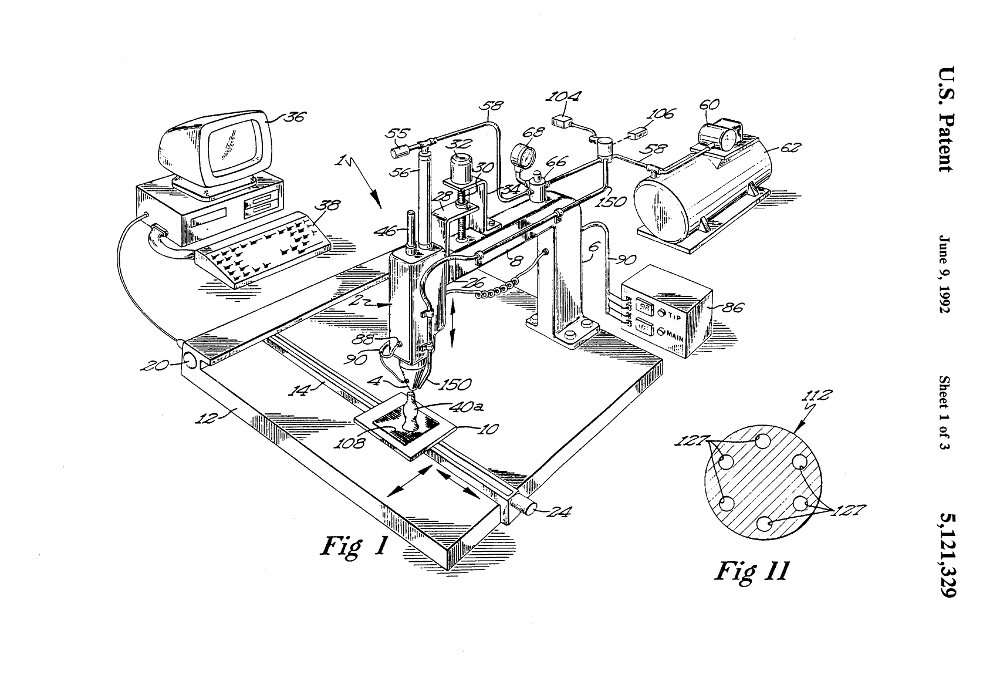
\includegraphics[width=\textwidth]{images/US5121329-1.png}
	\caption{US Patent 5121329}
	\label{img:us5121329a}
\end{figure}

\marginpar{The RepRap project works on creating general-purpose self-replicating
machines capable of printing plastic objects, and making them freely available
for the benefit of everyone.}

The surge of new cheap 3D printers -- as an affordable alternative to the large,
expensive industrial-grade machines -- was largely due to an increasing number
of enthusiasts from the \emph{Hacker-} and \emph{Maker-}Communities that worked
on projects like the RepRap\footnote{\url{http://reprap.org/wiki/RepRap}}, a
very successful and influential project.

As Erik De Bruijn, founder of the successful
Ultimaker\footnote{\url{https://www.ultimaker.com/}} company, discusses in his
Master's thesis \textit{``On the viability of the Open Source Development model
for the design of physical objects -- Lessons learned from the RepRap project''}
\cite{bruijn:2010}, the Open Source development model has proven to be well
suited in the field of physical fabrication.

At the same time, while many of these projects were started by communities as
non commercial Open Source\footnote{\url{http://opensource.org/}} and Open
Hardware\footnote{\url{http://www.oshwa.org/}} projects, crowdfunding platforms
like Kickstarter\footnote{\url{http://www.kickstarter.com/}} and
Indiegogo\footnote{\url{http://www.indiegogo.com/}} made raising capital for new
3D printers quick and easy, something that would not have been possible 10 years
ago. This resulted in a flood of readily assembled, affordable 3D printers even
for people lacking the skills to build their own machine from a list of parts.

%----------------------------------------------------------------------------------------

\section{From Data to Tangible Objects}

With the rapid and constantly accelerating developments in the field of 3D
printing, visualizing data as real, tangible objects has become feasible. There
are still some hurdles though.  The majority of people, even those owning a 3D
printer, have no experience with 3D modelling software. Most freely available
open source tools to create 3D models -- like OpenSCAD or
Blender\footnote{\url{http://www.blender.org/}} -- require a steep learning
curve and demand a nontrivial amount of learning time to create the desired
models. And platforms like
Thingiverse\footnote{\url{http://www.thingiverse.com/}} or
YouMagine\footnote{\url{https://www.youmagine.com/}} provide so many freely
available models that creating own objects is often not even a necessity.

Another aspect is that these general-purpose modelling tools are not optimized
for data visualization. Each type of visualization has to be created manually,
and when the data changes it's a lot of manual work to update the model.

\tangible{} was created to fill that void. It makes creation of customized,
printable data visualizations as 3D models easy, while at the same time
retaining a lot of flexibility for customization.
